\documentclass[9pt,twocolumn,twoside,lineno]{pnas-new}
\usepackage{multirow} %connecting columns in tables
\usepackage{multicol}
% Use the lineno option to display guide line numbers if required.
% Note that the use of elements such as single-column equations
% may affect the guide line number alignment. 

\templatetype{pnasresearcharticle} % Choose template 
% {pnasresearcharticle} = Template for a two-column research article
% {pnasmathematics} = Template for a one-column mathematics article
% {pnasinvited} = Template for a PNAS invited submission

\title{The scale of potential yield loss drives optimal management intensity in the face of evolving resistance}

% Use letters for affiliations, numbers to show equal authorship (if applicable) and to indicate the corresponding author

\author[a,1]{Shaun R. Coutts}
\author[a]{Helen L. Hicks} 
\author[b]{Alexa Varah}
\author[a]{Kwadjo Ahodo}
\author[a]{Rob Freckleton}
\author[a]{Dylan Z. Childs}

\affil[a]{Animal and Plant Sciences, University of Sheffield, Sheffield S10 2TN, UK}
\affil[b]{Zoological Society of London, London NW1 4RY, UK}

% Please give the surname of the lead author for the running footer
\leadauthor{Coutts} 

% Please add here a significance statement to explain the relevance of your work
\significancestatement{Integrated pest management (IPM) combines chemical and non-chemical control methods to pest populations to manage evolved resistance. Surprisingly, despite the widespread adoption of IPM, we have a poor understanding of how to select between alternative IPM strategies. Here we consider a typical farming system in which high levels of herbicide resistance evolves repeatedly. The best IPM strategies were dependent on crop yields, yield loss caused by the weed, the magnitude of the maximum possible loss, how future rewards are valued, and levels of herbicide resistance. With the exception of herbicide resistance, these factors are economic. Thus, knowing which IPM strategy to apply, and where to apply it, is both an economic and biological problem.}

% Please include corresponding author, author contribution and author declaration information
\authorcontributions{SRC conceived the idea did the modeling and wrote the initial draft. DZC contributed to the modeling. HLH collected field data for yield functions and aided in their interpretation. KA advised on economic cost modeling. All authors contributed to refining the focus and writing final manuscript.}
\authordeclaration{No conflicts of interest.}
\correspondingauthor{\textsuperscript{1}To whom correspondence should be addressed. E-mail: shaun.coutts\@gmail.com}

% Keywords are not mandatory, but authors are strongly encouraged to provide them. If provided, please include two to five keywords, separated by the pipe symbol, e.g:
\keywords{Integrated Pest Management $|$ herbicide resistance $|$ \textit{Alopecurus myosuroides} $|$ combinatorial optimization} 

\begin{abstract}
Evolved resistance to xenobiotics (e.g.\ antibiotics, herbicides, insecticides, fungicides) is a global threat to public health and food security. In agricultural systems, non-chemical control methods can be combined with xenobiotics (Integrated Pest Management; IPM) to prolong the useful life of compounds and manage pest populations after resistance has evolved. However, finding cost effective IPM strategies is challenging due to the large number of possible strategies, many of which will perform poorly. In order for IPM strategies to be adopted by farmers and used over the long-term they need to balance the short-term gains of repeatedly using the most cost-effective tool (often chemical control), against long term losses from evolved resistance. We find IPM strategies with the highest economic returns for an arable cropping system and perform a global sensitivity analysis to find the factors that shape those strategies. The key uncertainties are economic in nature, and farmers have an incentive to be responsive to changes in weed density and the effect of the weed on yield. Doing so effectively will require estimating, at a minimum, what yields would be in the absence of the weed, maximum weed density and how yields change with increasing weed density, with enough detail to say how much control (if any) is justified. The ultimate solution to xenobiotic resistance will require reducing their use. Any strategy that achieves this at scale must recognize when the intensive use of xenobiotics is incentiveized, and also when a more diverse IPM strategy is favored.   
\end{abstract}

\dates{This manuscript was compiled on \today}
\doi{\url{www.pnas.org/cgi/doi/10.1073/pnas.XXXXXXXXXX}}

\begin{document}

% Optional adjustment to line up main text (after abstract) of first page with line numbers, when using both lineno and twocolumn options.
% You should only change this length when you've finalised the article contents.
\verticaladjustment{-2pt}

\maketitle
\thispagestyle{firststyle}
\ifthenelse{\boolean{shortarticle}}{\ifthenelse{\boolean{singlecolumn}}{\abscontentformatted}{\abscontent}}{}

%Introduction
\dropcap{C}ontrolling populations in the face of evolving resistance to xenobiotics (i.e.\ antibiotics, herbicides, pesticides, fungicides) is one of the biggest challenges facing public health \citep{Laxm2016, Willy2017}, and food security \citep{Denh1992, Palu2001, Hick2018}. Evolved resistance also costs billions of dollars globally \citep{Livi2016, Ches2018, Hick2018}. In agricultural systems evolved resistance can be mitigated against through integrated pest management (IPM), where chemical control is used in combination with non-chemical techniques such as crop rotation, cultivation and spot control (e.g.\ hand-weeding). IPM can be used both pro-actively to delay the evolution of resistance, and reactively to control pest populations as chemical control becomes less effective \citep{Denh1992, Hick2018}. While most current strategies focus on delaying resistance \citep{REX2013}, in many agricultural weeds herbicide resistance is already widespread \citep{Jord1997, Samm2014, Hick2018}. Thus, cost effective IPM strategies focusing on managing weeds in the face of existing resistance are needed.               

While the concept of IPM is well established \citep{Bott1979}, for IPM strategies to be adopted by farmers, and used long-term, they must be economically viable \citep{Hurl2016}. Finding cost effective IPM strategies is extremely challenging \citep{Dana2014, Chal2015}. Management tools need to be used in the correct combination and sequence to be effective. This results in a very large number of potential IPM strategies (i.e.\ different combinations and sequences), even when considering only a handful of management tools and short time horizons \citep{Chal2015}. In addition, weed populations are ecologically and evolutionarily dynamic, responding to any management options used. As a result of this difficulty, there have been no attempts to rigorously search for cost effective IPM strategies in the face of rapidly evolving resistance to key chemical controls. This is an important gap in our understanding for agricultural systems, in which resistance to xenobiotics has evolved numerous times \citep{Denh1992, Palu2001, Samm2014} and multiple non-chemical control options can be used in combination to deliver cost effective control \citep{Lutm2013}.      

Finding economically incentivised IPM strategies is made more difficult in the face of evolving resistance by spatial and temporal variation weed population dynamics and socio-economic factors. Firstly, the benefits of weed control are challenging to estimate. One must estimate both the effect of a weed control tool on the weed population, and also the effect of different weed densities on crop yield, called the yield loss function. While yield loss functions have been estimated for decades \citep{Blea1960, Cous1985}, there can be considerable variation in yield loss functions between fields \citep{Swin1994}, and yield loss functions for particular fields are often unknown. Secondly, the way future rewards are valued (i.e. discounted) can have a large effect on long term investments like weed control \citep{Wies1996, Fras2004}. The way future rewards are valued can vary between farmers due to personal traits like appetite for risk, or systemic factors like land tenure \citep{Fras2004}. Economically viable IPM strategies must, therefore, balance the short-term gains of repeatedly using chemical control (often the most cost effective tool), against future loses that result from evolved resistance \citep{Hick2018}. To do this IPM strategies will need to consider both costs and benefits, how they change in the face of evolving resistance, and how they are valued in the future.  
        
Little is known about how robust good IPM strategies are to changes in factors such as crop yield and pest population dynamics \citep{EpanN2010}. Thus, even when effective IPM strategies are found, we do not know how generally they should apply. Robust IPM strategies would allow standard IPM strategies to be developed for entire farms or regions. If robust IPM strategies cannot be identified then farmers face the prospect of having to find workable IPM strategies for each economic and biological scenario. This would pose a serious barrier to IPM adoption, as IPM strategies are already seen as complex and difficult to implement \citep{Llew2006}. An alternative is to find a small number of cost-effective IPM strategies and a set of easily measurable factors that allow farmers to choose between them.

We framed IPM as a combinatorial optimization problem and used a genetic algorithm (Appendix 1) to find economically incentivized (measured by gross margin) IPM strategies \citep{Tayl2004GA, Carr2010} in the face of evolution. \textit{Alopecurus myosuroides} was used as a test case. Herbicide-resistant \textit{A.\ myosuroides} costs up to \pounds 320$\cdot$ha$^{-1}$ in yield loss and extra herbicide use \citep{Hick2018}, is one of Europe's most economically costly weeds \citep{Moss2007}, and one of the world's most serious herbicide resistant weeds \citep{Heap2014}. We modeled a population of \textit{A. myosuroides} in which target site resistance to two herbicides is already present, although possibly at very low frequencies. To allow non-chemical control in the IPM strategies the population model has two seed bank levels so that cultivation can bury seeds, and spring crops and spot control (e.g. by hand weeding) affect survival. We carried out a global sensitivity analysis (Appendix 2), testing how robust those IPM strategies were across 15,000 parameter combinations incorporating a wide range of economic, biological and psychological factors. We find that cost effective IPM strategies can change dramatically in response to changes in potential yield losses, but those changes are predictable. 

\section*{Results and Discussion}
Across a wide range of parameter combinations the most important parameters shaping IPM strategies relate to the immediate, or potential maximum, economic impact of the weed. In particular parameters defining the yield loss function (Fig.\ \ref{fig:rel_inf}a) have the most influence on shaping incentivized IPM strategies. The yield loss function describes the relationship between weed density and crop yield (Fig.\ \ref{fig:rel_inf}b). Yield when the weed was absent ($Y_0$) and the effect of weed density on yield ($Y_D$) were two of the most important parameters (Fig.\ \ref{fig:rel_inf}). The set of parameters that controls the potential size of the seed bank ($f_m$, $f_d$ and $\phi_b$; Fig.\ \ref{fig:rel_inf}a), and therefore the the maximum possible loss if the weed population is uncontrolled (Fig.\ \ref{fig:rel_inf}b), are also important. Although yield loss functions have been estimated for major weeds \citep{Cous1985, Doyl1986, Swin1994}, there is evidence that yield functions vary substantially between fields \citep{Swin1994, Hick2018}, and little attention has been paid to this variation and understanding its causes.
 \begin{figure}
	\centering
	\includegraphics[width=75mm]{rel_inf_yield_func.pdf}
	\caption{a) Relative influence of each parameter on IPM strategy. Higher values indicate parameters with more influence on the structure of incentivized IPM strategies. To find which parameters were crucial in shaping IPM with high gross margin we used multi-variate boosted regression trees \citep{Mill2016} as a meta-model \citep{Cout2014}(Appendix 2). We interrogated this meta-model to find important parameters accounting for high-level interactions and non-linear responses \citep{Frie2001, Mill2016}. Relative influence is the reduction in mean squared error attributable to each parameter. Because only relative values are only meaningful the index is re-scaled to sum to 100 across all parameters \citep{Frie2001}. b) The most important parameters are related to the yield loss function. We use a linear yield function fit to empirical data (Appendix 3).}
	\label{fig:rel_inf} 
\end{figure}

The shape of the yield loss function is important because it determines how much control is justified. However, knowing which type of IPM strategy to employ may only require an estimate of the pest free yield ($Y_0$), and one or two threshold values of weed density where a new IPM strategy becomes advantageous:
\begin{enumerate}
	\item When the yield of winter wheat in the absence of \textit{A.\ myosuroides} ($Y_0$) is low, management intensity is lower and relies on crop rotation and tactical use of herbicide (Fig.\ \ref{fig:Y0_YD}, '$Y_0$ low').
	\item The strategy changes little when the effect of weed density on yield ($Y_D$) increases. However, more herbicide is used when the value of $Y_D$ increases from a very low value to a slightly higher value (1\% to 12\% losses at high densities of \textit{A.\ myosuroides}; Fig.\ \ref{fig:Y0_YD}g,e). 
\end{enumerate}
When $Y_0$ is high, $Y_D$ shows two thresholds where IPM strategy changes. 
\begin{enumerate}
	\item When $Y_D$ is very low, even the maximum \textit{A.\ myosuroides} population does not cause yield losses high enough to justify expenditure on control and the best strategy is to do nothing (Fig.\ \ref{fig:Y0_YD}h).
	\item When $Y_D$ increases slightly the IPM strategy shifts to a simple management regime of intermediate intensity (Fig.\ \ref{fig:Y0_YD}f). 
	\item Once $Y_D$ increased enough to justify intensive control, further increases did not change the IPM strategy (Fig.\ \ref{fig:Y0_YD}b,d).    
\end{enumerate}
 
\begin{figure}
	\centering
	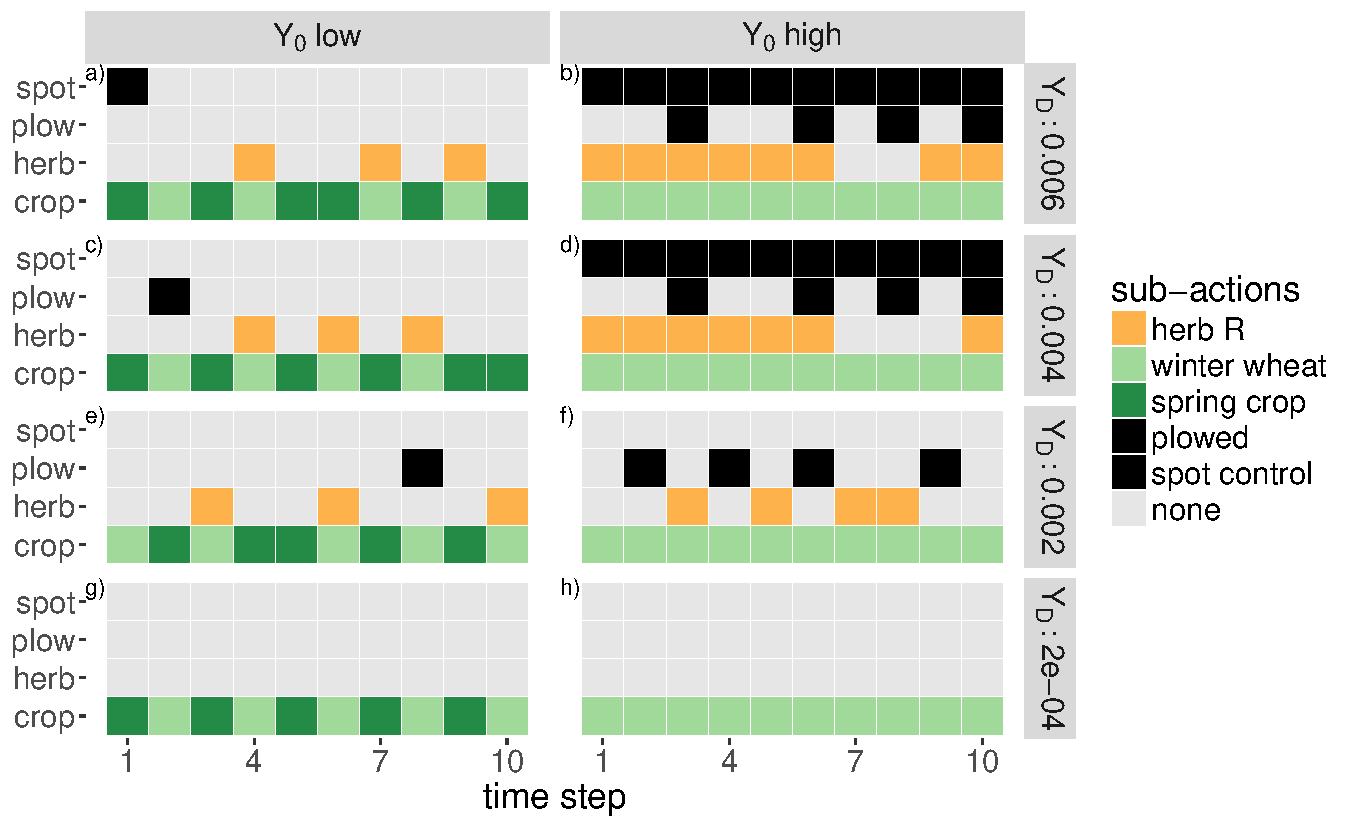
\includegraphics[width=1\linewidth]{MS_act_seq_YD_Y0.pdf}
	\caption{IPM strategies under high (\pounds 1668$\cdot$ha$^{-1}$) and low (\pounds 986$\cdot$ha$^{-1}$) values of $Y_0$ (yield of winter wheat with no \textit{A. myosuroides}), under increasing values (rows) of $Y_D$ (in \pounds$\cdot$plant$^{-1}\cdot$ha$^{-1}$). At the lower limit of $Y_D$ very high \textit{A.\ myosuroides} densities result in a 1\% yield loss under the high $Y_0$ scenario, and the upper limit implies a yield loss of 35\%. There is initially one effective herbicide ($R_\text{int} = 0.0001$, $Q_\text{int} = 0.9$). Sub-actions are: crop (winter wheat or spring barley), herbicide (herb R, resistance conferred by allele $R$), plow (to plough or not), spot (to carry out spot control or not). We used partial dependence plots to explore how different parameter combinations change IPM strategy. Partial dependence plots show the marginal effect of a parameter of interest on IPM strategy \citep{Frie2001, Mill2016}. Once relevant parameter ranges were found we re-ran the genetic algorithm for those parameter combinations to generate actual IPM strategies rather than the marginal effects.}
	\label{fig:Y0_YD} 
\end{figure}

Historically, farmers do not change their management in response to yield losses, and apply the same amount of herbicide (the primary management tool in this system) regardless of the impact weeds have on crop yields \citep{Hick2018}. This is a potentially expensive choice, as farmers my incur management costs with no reward, and then suffer high costs from yield loss if weed populations increase \citep{Hick2018}.         

Intensive management is costly, and so requires returns over several years to justify. As a result, valuing returns further into the future encourages more intensive management \citep{EpanN2010}. Intensive management to reduce the seed bank is only selected by the genetic algorithm when future returns are given more value (higher values of the discount rate, $\gamma$, Fig.\ \ref{fig:dis_rate}). In agricultural systems land tenure has a crucial effect on how investments in weed control are valued. Those who own fields can benefit from long-term investments like weed control campaigns and soil conservation, whereas those who rent fields do not \citep{Wies1996, Fras2004}. The amount of rented farm land can be considerable. 54\% of crop land in the USA is rented \citep{Bige2016}, as is 35\% of all agricultural land in England and Wales \citep{CAAV2017}. This has important implications for the level of control managers are incentivized to provide, and thus the spread and the evolution of resistance \citep{Mare2012}. When crop yields are low the time to pay back investments in weed control increases, and future returns have to be valued even more highly to justify intensive control to drive down the seed bank (Fig.\ \ref{fig:dis_rate}b). Thus, the effect of land tenure on weed populations at landscape scales may be less pronounced when crop yields are high, as even people with relativity low discounts rates are incentivized to control (Fig.\ \ref{fig:dis_rate}a).

\begin{figure*}
	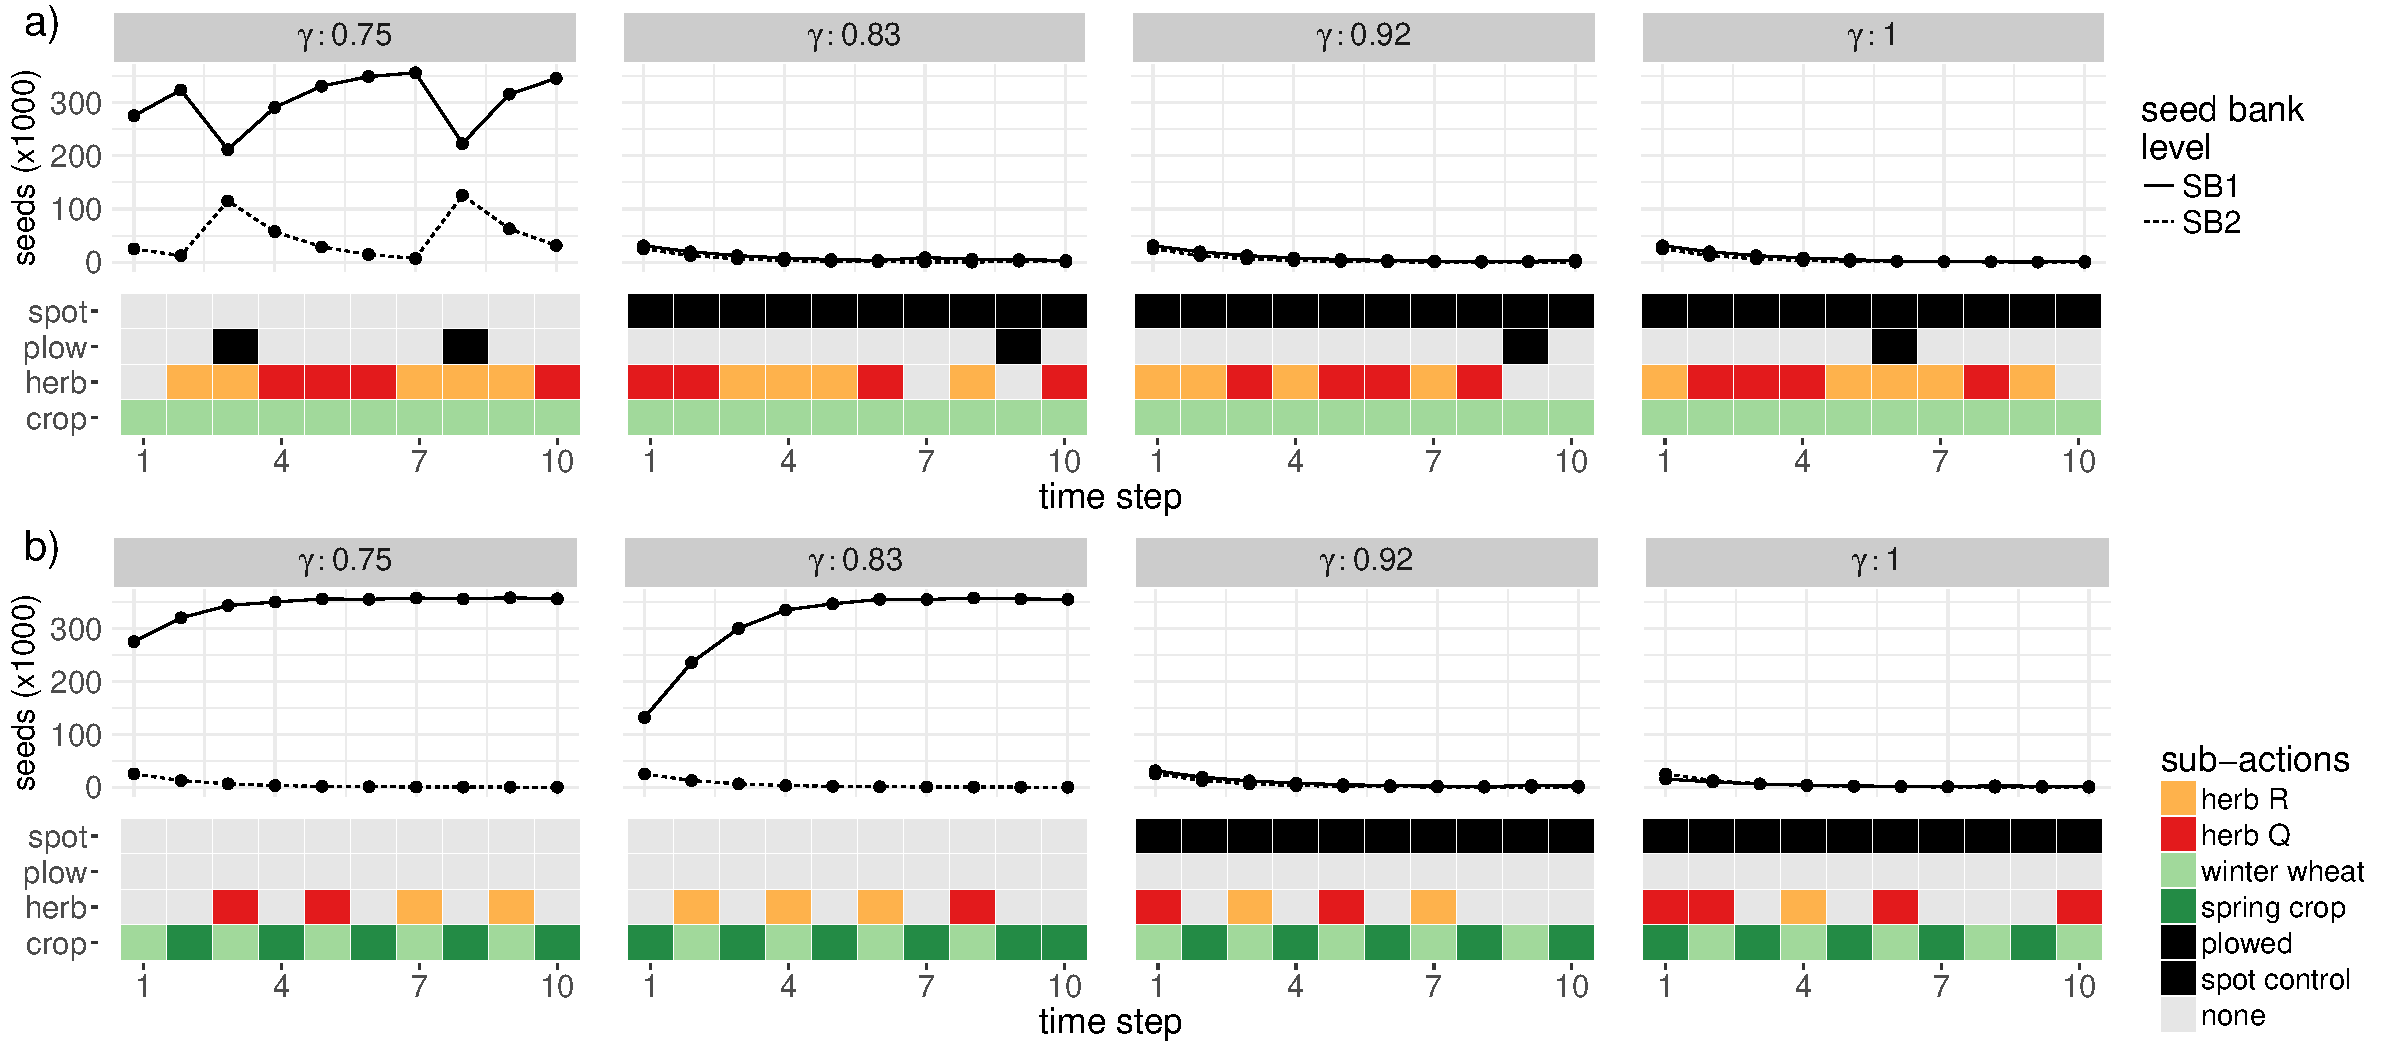
\includegraphics[width=178mm]{dis_rate_SB_strat.pdf}
	\caption{The effect of discount rate ($\gamma$) on the seed bank and IPM strategy (tile plots) when yields from winter wheat are high (a; \pounds 1668$\cdot$ha$^{-1}$) and low (b; \pounds 986$\cdot$ha$^{-1}$). When $\gamma = 0.75$ rewards 5 years in the future are valued at 23\% of current returns and when $\gamma = 1$ present and future rewards are valued equally. In both cases the slope of the yield function ($Y_D$) is high (\pounds 0.006$\cdot$plant$^{-1}\cdot$ha$^{-1}$). Sub-actions are: crop (winter wheat or spring barley), herbicide (herb R/Q, resistance conferred by allele $R$ or $Q$), plow (to plough or not), spot (to carry out spot control or not). All seeds enter, and germination occurs from, the top level of the seed bank (SB1). Seeds only enter the lower seed bank level SB2 through ploughing. Initial resistance was low for both herbicides. Although we only show the first 10 years of IPM strategy, the discounted returns over 25 years are considered by the genetic algorithm.}
	\label{fig:dis_rate} 
\end{figure*}

Resistance increases quickly with herbicide use. Even starting at low frequencies (TSR allele $Q$ starting frequency 1 in 20000), high levels of resistance evolves after just seven herbicide applications (Fig.\ \ref{fig:int_res}b). In our system herbicide resistance incurs a high cost, reducing gross margin (reward) by up to a quarter once high levels of resistance evolve (Fig.\ \ref{fig:int_res}c,d). As a result, the best IPM strategies are responsive to increasing resistance, drastically reducing herbicide use as higher levels of resistance evolve (Fig.\ \ref{fig:int_res}b--d). In contrast, multiple herbicide applications per year are the norm in this cropping system, despite high levels of resistance \citep{Hick2018}. This disparity could arise from a number of contributing factors. Some managers may believe that even a little control (mortality of a few susceptible individuals) is better than no control and inaction is seen as the worst approach to weed management \citep{Wils2008}. In addition, IPM strategies are often seen as complex and more difficult to implement than the routine application of chemicals \citep{Llew2006}. There may be a belief that new herbicides will become available \citep{Hurl2016}, despite no new modes of action being marketed for over 20 years \citep{Duke2012}. Finally, uncertainty in the efficacy of non-chemical control is a major impediment to adopting IPM, and farmers may prefer to stick with known chemical control, even if it is only partially effective \citep{Hurl2016}.

Over a wide range of parameters, when both herbicides are effective the preference is to cycle herbicides (using different compounds sequentially; e.g. Fig.\ \ref{fig:dis_rate} and \ref{fig:int_res}a) rather than stacking them (using different compounds at the same time). Cycling is favored over stacking because the application of each herbicide is reduced, prolonging their useful life, without reducing the number of times herbicide was applied. An important assumption behind this result is that we modeled reactive management, where resistant genotypes are already established in the population \citep{Hick2018}. In contrast, much work on managing resistance focuses on proactive management, delaying the initial \textit{de nova} evolution of resistance. In proactive management both stacking and cycling can be effective \citep{REX2013}. We present the best case that can be hoped for in reactive management, as we assume that herbicide resistance was conferred by target site mutations. There is growing evidence that non-target site resistance, which frequently confers cross resistance, is widespread \citep{Hick2018}. If generalized, non-target site resistance mechanisms are present, the total amount of herbicide exposure predicts resistance level \citep{Hick2018}, and cycling is unlikely to slow the evolution of resistance. 
\begin{figure*}[!ht]
	\includegraphics[width=178mm]{int_res_strat_resist_edit.pdf}
	\caption{The effect of initial resistance to herbicide R (resistance conferred by allele R) and herbicide Q on the selected IPM strategy (tile plots) and the evolution of herbicide resistance (\% survival to under both herbicides). Lighter colored points indicate higher reward (gross margin) obtained in that time step. In both cases the slope of the yield function ($Y_D$) is high (\pounds 0.006$\cdot$plant$^{-1}\cdot$ha$^{-1}$). Sub-actions are: crop (winter wheat or spring barley), herbicide (herb R/Q, resistance conferred by allele $R$ or $Q$), plow (to plough or not), spot (to carry out spot control or not). In this case $Y_0 = 1668$ (high winter wheat yield) and $Y_D = 0.0062$ (high yield penalty).}
	\label{fig:int_res} 
\end{figure*}

We assume that herbicide is the only action that drives the evolution of resistance. Relaxing this assumption would be an important extension. Any effective management tool will impose selection pressure, and so drive resistance to that tool \citep{Jord1997}. For example, in our system spring cropping and spot control make heavy use of glyphosate, and glyphosate resistance has evolved repeatedly in response to prolonged, heavy use \citep{Samm2014}. 

\section*{Conclusion}
The eventual solution to pesticide resistance will require reducing their use. Any strategy to drive this behavior change at scale will need to mitigate farmers economic incentives where they encourage short-term intensive use of pesticides. Where such intensive use is sub-optimal, for example when high levels of resistance have already evolved, other factors encouraging continued over-use, such as land tenure \citep{Fras2004} and social norms that favor action over inaction \citep{Wils2008}, will need to be recognized and addressed. Existing tools from the social sciences can help map out community wide strategies in response to complex, society wide challenges when a sufficient knowledge base around the problem exists \citep{Barn2014}. We argue that for resistance in agricultural systems this knowledge base is feasible to build. 

Economically incentiveized IPM strategies fall on a well defined continuum from little or no management, up to intensive management. A small number of parameters, mainly defining the yield loss function, determined where the best IPM strategy sits on this continuum. Thus, farmers have an economic incentive to be responsive to changes in the shape of the yield loss function. Doing so will require estimating, at a minimum, what yields would be in the absence of the pest, and how yields change with increasing pest density, with enough detail to say how much control (if any) is justified. The most salient piece of data on the weed population is its maximum density, as this sets yield loss in the absence of management. 
  
The alternative is to maintain the current management paradigm in spite of herbicide resistant weeds, which could cost hundreds of millions annually in extra control costs and yield losses \citep{Hick2018}. This presents a substantial economic incentive to identify thresholds at which a new IPM strategies become advantageous. Finding such thresholds will be an ongoing research project as new threats arise. But tools for rapidly mapping weed populations \citep{Quee2011, Lamb2018} and measuring yield at fine scales (e.g.\ modern harvesters) will allow us to find yield loss functions at landscape scales. 

\subsection*{Data Archival}
Data used to fit the yield function and model code can be accessed at University of Sheffield Research Data Repository.

\subsection*{Supporting Information (SI)}
\subsubsection*{Appendices}
Appendix 1: Genetic Algorithm\\
Appendix 2: Finding Which Initial Conditions and Model Parameters Lead to Which IPM Strategies\\
Appendix 3: Reward Function\\
Appendix 4: Action Space\\
Appendix 5: Population Model\\

%METHODS
\matmethods{We frame IPM as a combinatorial optimization problem where the goal is to find a good combination of management tools, used in sequence. We use a genetic algorithm to solve this combinatorial problem \citep{Tayl2004GA, Carr2010}. Genetic algorithms cannot be checked to have found the globally optimal solution, as this would require already knowing the solution; however, genetic algorithms are efficient at selecting out comparatively poor solutions, so that over successive iterations the regions of the solution space being explored gets progressively better, resulting in a set of good (often near optimal) solutions.

Our goal is to find good IPM strategies in the face of rapidly evolving resistance, and how those strategies change in response to biological and management parameters. This problem has fours parts: i) a reward function that measures how good a given IPM strategy is based on how much that strategy costs and its effectiveness, we use time discounted gross margin \citep{Nix2016}; ii) a population model that translates a given IPM strategy into a population, and thus a reward; iii) an algorithm that finds IPM strategies with higher rewards, the genetic algorithm (Appendix 1); iv) finally we need to relate changes in the best IPM strategy found to changes in initial conditions and model parameters. For this we use a meta-modelling global sensitivity analysis \citep{Cout2014} based on multi-variate boosted regression trees \citep{Mill2016}. 

\subsection*{Population model}
The population model links management actions to the response of the \textit{A.\ myosuroides} population, and thus wheat yields. Each action $a_j$ is a tuple of four sub-actions $a_j = \langle a_h, a_b, a_k, a_s \rangle$. See Appendix 4 for a description of the sub-actions and all eligible combinations of these sub-actions (i.e.\ the full actions space, $\mathbf{A}$). 

The processes included in the population model limit the scope of the IPM strategies found. We use a deterministic model, and so our IPM strategies can only deal with average expected population responses, ignoring demographic uncertainty, and environmental and market variability. Also, we only model herbicide resistance that is already present in the population because \textit{de nova} mutation is a fundamentally stochastic process. 

A commonly recommended \citep{REX2013} and applied \citep{Hick2018} strategy to combat resistance is to apply xenobiotics that impair different cellar pathways (i.e. modes of action), either sequentially (cycling) or concurrently (stacking). To allow this behavior we use a discrete time, spatially implicit model, where two independent alleles ($R$ and $Q$), each confer target site resistance to a separate herbicide. The model must also be flexible enough to accommodate non-chemical control. We include a two level seed bank (to allow plowing to take seeds out of the germinating population) and model survival as a function of resistance, herbicide choice, crop choice and spot control (where the cost increases with \textit{A.\ myosuroides} density). The model tracks the number of seeds in each level of the seed bank in each of nine genotypes $G$, starting at the beginning of the growing season before any seeds have emerged. See Appendix 5 for a full description of the model and how each sub-action affects the population. 

\subsection*{Reward function}
The reward function measures how good an IPM strategy is, given an initial starting condition and parameter set that the model is run under. The reward function encodes the goals of a manager. We assume farmers are primarily driven by economic returns. The economic return consists of two parts: the income made from the crop, and the costs of producing that crop. We assume that usual farm costs, such as buildings and machinery are constant from year to year, so we focus on gross margin, i.e. income - variable costs \citep[pp.~3--4]{Nix2016}. 

To explicitly link the above ground population to the reward function we define $N''(\mathbf{a}, n_0, t)$, the total above ground population in time $t$ after all sub-actions have been carried out, given an initial population $n_0$ and a sequence of actions 
\begin{equation}
	\mathbf{a} = \{a_j^0, a_j^1, \cdots, a_j^T\}
\end{equation}	  
where $a_j^t$ is the action $a_j \in \mathbf{A}$ taken at time $t$ and $T$ is the time horizon over which management is run. We assume all returns after $T$ are ignored. The reward function is  
\begin{equation}
	R(\mathbf{a}, n_0) = \sum_{t=0}^T \gamma^t \Big( Y(N''(\mathbf{a}, n_0, t)) - C(a_j^t) \Big)
\end{equation}
where $R(\mathbf{a}, n_0)$ is the time-discounted reward for action sequence $\mathbf{a}$ given starting population $n_0$, $\gamma \in [0, 1]$ is the discount rate. When $\gamma = 0$ only the reward in the first time step is considered; when $\gamma = 1$ returns in all future time steps up to $T$ are valued equally. $Y(N''(\mathbf{a}, n_0, t))$ is the income (in \pounds$\cdot$ha$^{-1}$) from the crop chosen at time $t$ given initial state $n_0$ and following action sequence $\mathbf{a}$. $C(a_j)$ is the cost of taking action $a_j$, and is composed of the cost of controlling \textit{A.\ myosuroides} plus other costs that depend on the crop being grown ($a_k$).   

See Appendix 3 for the yield and cost models for each sub-action and parameter estimation.

\subsection*{Finding good IPM strategies} 
It is not feasible to test every combination of management options over more than a handful of years. Genetic algorithms have been used to find good solutions to this class of problem \citep{Tayl2004GA, Carr2010}. The genetic algorithm starts with an randomly generated set of action sequences. These action sequences are then iteratively improved to find a set of action sequences with a high gross margin. Genetic algorithms rely on the fact that even though the number of possible action sequences is large, many perform very poorly. The genetic algorithm explores better performing regions of the solution space more intensely. While genetic algorithms are not guaranteed to find the optimal action sequence they will find a set of actions sequences that perform well, often close to the optimal solution.   

To find good action sequences we use a genetic algorithm with knock-out tournament selection, where each action sequence in a set of 1000 actions sequences is randomly paired with another, and the action sequence with the highest $R(\mathbf{a}, n_0)$ survives to help generate new action sequences. We used pair mating between survivors and N-point cross-over to produce new action sequences. After new action sequences are created there is a process of random mutation where each $a_j^t$ is changed to another $a_j^t \in \mathbf{A}$ with probability $m = 0.03$. The algorithm used is given in Appendix 1.        

\subsection*{Finding which initial conditions and model parameters lead to which IPM strategies}
It is unlikely a given IPM strategy will perform well in all scenarios. To find the parameters and initial conditions ($n_0$) that shaped the IPM strategy with the highest reward, we extend the meta-modelling approach to global sensitivity analysis (outlined in \citep{Cout2014}), to multivariate time series outputs (i.e. the sequences of the four sub actions). We: i) ran the genetic algorithm under 15000 different parameter sets and initial conditions, generated with Latin hyper-cube sampling (see Table S1 in Appendix 2 for upper and lower limits of each parameter); ii) used Longest Common Sub-Sequence \citep{Tooh2015} as a measure of distance between these action sequences; iii) projected the resulting distance matrix into an 8D solution space using non-metric multi-dimensional scaling, implemented in the 'ecodist' R package \citep{Gosl2007}; and iv) predicted where each IPM solution sat in the solution space using multi-variate boosted regression trees \citep{Mill2016}, where the model parameters and initial conditions were predictors. See Appendix 2 for details.

We interrogated this multi-variate boosted regression tree to find which parameters and initial conditions were important for changing the best IPM strategy found. We used two tools, relative influence and partial dependence plots \citep{Mill2016}.    
}

\showmatmethods % Display the Materials and Methods section

\acknow{We thank the BGRI Farmer Focus group for valuable insight on IPM strategies.}

\showacknow % Display the acknowledgments section

% \pnasbreak splits and balances the columns before the references.
% If you see unexpected formatting errors, try commenting out this line
% as it can run into problems with floats and footnotes on the final page.
%\pnasbreak

% Bibliography
\bibliography{biblio_refs} 

\end{document}